\section{Sequenced semantics in a \\ distributed environment}
\label{sec:consider}

\eat{Sequenced semantics has three properties: snapshot reducibility,
extended snapshot reducibility, and change
preservation~\cite{Dignos2012}.  }

Our goal is to enable querying and analysis of large evolving graphs
with sequenced semantics in a distributed environment.  Many
interesting static graphs are so large that they necessitate a
distributed approach, as evidenced by the plethora of works on
Pregel-like computation and graph partitioning~\cite{McCune2015}.  All
three properties of sequenced semantics -- snapshot reducibility,
extended snapshot reducibility, and change preservation -- must be
supported despite the distributed nature of the computation.

\eat{With the added time dimension, efficient computation over graphs with
sequenced semantics presents three challenges:}

\eat{
\begin{enumerate}
\item How to partition temporal relations optimally.
\item How to support sequenced semantics over a partitioned relation.
\item How to partition a large evolving graph such that both temporal
  and structural locality is balanced.
\end{enumerate}}

\begin{figure}
\begin{subfigure}[b]{1.6in}
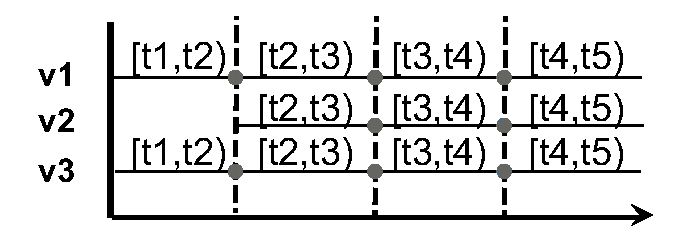
\includegraphics[width=1.6in]{figs/split.pdf}
\caption{with fragments}
\vspace{-0.2cm}
\label{fig:split}
\end{subfigure}
\begin{subfigure}[b]{1.6in}
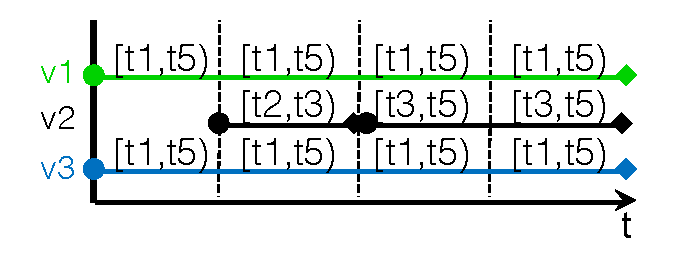
\includegraphics[width=1.6in]{figs/split2.pdf}
\caption{with full timestamps}
\vspace{-0.2cm}
\label{fig:split2}
\end{subfigure}
%\caption{Relation V from Figure~\ref{fig:coalesced} split in 4 partitions.}
\caption{Vertices from Figure~\ref{fig:snapshots} split in 4 partitions.}
\vspace{-0.5cm}
\end{figure}

{\bf Snapshot reducibility.}  Evolving graphs can be partitioned among
the available instances using time locality.  Following convention, we
refer to the operator that can produce such partitioning as a {\em
  splitter}.  The splitter places each tuple (vertex or edge) into one
or more partitions based on its timestamp.  The goal of the splitter
is to form partitions that are balanced, i.e., have approximately the
same number of items, under the assumption that most operations can be
executed locally at each partition.  Recall that snapshot reducibility
requires a temporal operator to produce the same result as if it were
evaluated over each snapshot.  Validity period of a tuple that spans
more than one temporal partition is split, and the tuple is replicated
across partitions.  This increases the overall size of the relation,
but all operations can now be carried out within each partition.  See
Figure~\ref{fig:split} for a simple example of the $V$ relation being
split into four temporal partitions.  

For the purposes of illustration, consider a temporal subgraph
operation, a generalization of subgraph matching for non-temporal
graphs.  Temporal vertex-subgraph \subv{q^t_v}{\ttt} computes an
induced subgraph of \tve $\tve'(\tv', \te', \tav', \tae')$, with
vertices defined by the temporal conjunctive query $q^t_v$.  Note that
this is a subgraph query, and so $\tv' \subseteq^T \tv$.  Observe that
we can carry out a subgraph operation with predicate
\insql{name='Alice'} at each partition individually, without any
cross-partition communication.

The question of optimal splitting has been addressed by Le et
al.~\cite{Le2013}, who demonstrated that a temporal relation can be
efficiently split into $k$ buckets in cases of both internal memory
and external memory and guarantee optimality of solution\eat{in $O(N
  log N)$ time in internal memory and in $O(SORT(N)$ I/Os in external
  memory}.  This method requires a sequential scan of the relation to
compute an index called the stabbing array.  How to make this method
more efficient in a distributed environment is an open question.

\eat{ However, Le's approach is not the most efficient in a
distributed environment because it requires a sequential scan of the
relation to compute the stabbing array.  We have found an approach
that is parallelizable (no sequential scan) and completes in $O(N*m)$
time, where $N$ is the size of the relation and $m$ is the number of
distinct starting values.  In typical evolving graphs this $m$ is
significantly smaller than $log n$ and is thus faster than Le's
approach with and without parallelization.}

A number of alternatives for co-partitioning of graph relations
present themselves, as the vertex and edge relations are not
guaranteed to have the same splitters due to different evolution
rates.  Typically, vertices are co-partitioned with edges in the
non-temporal case~\cite{DBLP:conf/osdi/GonzalezXDCFS14}, and this
likely is most efficient with evolving graphs as well.  The subgraph
operation requires such co-partitioning to enforce referential
integrity on edges.

\eat{
Temporal partitioning is also appropriate for binary operators as long
as the two input relations are partitioned together, i.e., have the
same splitters.}  
\eat{Because each entity (vertex or edge) evolves at
  a different rate, the boundaries of partitions will require
  splitting of some of the tuples such that they reside in more than
  one partition.}  
\eat{An open question is what to do when a binary
operator is applied to two relations that are already partitioned
independently -- it may be more efficient to repartition one of them
using the splitters of the other, or apply the operator over existing
partitions and accept the cost of cross-partition communication.}

\eat{{\bf Temporal partitioning.}  In temporal algebra with point
semantics all queries can be carried out independently at each time
partition, which means that the cross-partition communication is not
necessary.  }

\eat{As long as the full timestamp is
preserved in each fragment after the split, both the snapshot
reducibility and extended snapshot reducibility properties are
observed using the approach in~\cite{Dignos2012}.}  

{\bf Extended snapshot reducibility.}  Snapshot reducibility can be
guaranteed in the distributed setting, as shown above.  \eat{Extended
  snapshot reducibility and change preservation require additional
  work.  }Subgraph query $q^t_v$ may use any of the constituent
relations of \tve, and may explicitly reference temporal information
in compliance with the extended snapshot reducibility property of
sequenced semantics.  Refer back to Figure~\ref{fig:split} and assume
time granularity of years.  If we perform a subgraph operation with a
temporal predicate such as \insql{p > 2 years} over the split, then we
will get no matches.  However, the original relation contains two
matches -- only Bob \eat{with \insql{vid=2} }does not meet the
predicate.  To support extended snapshot reducibility over a split
relation, during partitioning tuples should be placed into their
partitions with their full original timestamps.  Incidentally, this is
what Le at al. describe in their work on optimal
splitters~\cite{Le2013}.  Figure~\ref{fig:split2} shows relation $V$
split in the same four partitions with this approach.

{\bf Change preservation.}  Change preservation property requires that
derived tuples should only be coalesced if they share lineage.  To
support this property, a normalize and align operators are used.  The
normalize operator splits each tuple in the input relation w.r.t. a
group of tuples such that each timestamp fragment is either fully
contained or disjoint with every timestamp in the group.  The align
operator splits each tuple w.r.t. a group of tuples such that each
timestamp fragment is either an intersection with one of the tuples in
the group or is not covered by any tuple in a group.\eat{ (See Figure
  2 in~\cite{Dignos2012} for an illustration.)}

The normalize operator splits each tuple w.r.t. to a group defined by
the operation.  For example, consider an attribute-based node creation
operation on graphs, similar to aggregation on temporal relations.
This operation allows the user to generate a \tg in which vertices
correspond to disjoint groups of vertices in the input that agree on
the values of all grouping attributes.  For instance,
$\insql{node}^T_a(school,\tve)$ will compute a vertex for each value
of $\tav.a.school$.  While the group defined for each tuple (distinct
value of $school$) spans temporal partitions, only tuples within the
same partitions overlap.  Thus the normalize operation can be carried
out at each partition locally.  Similarly for the align operator.

{\bf Spatio-temporal partitioning.}  Large evolving graphs present
additional challenges compared to static graphs and temporal relations
alone.  Each graph snapshot may be too large to fit into a single
partition.  This necessitates partitioning graphs by both time and
structure.  Miao et al.~\cite{Miao2015} have demonstrated within their
ImmortalGraph system that different locality, structural or temporal,
is more appropriate for different graph queries.  However, the results
do not directly translate into the distributed environment because of
the parallelism gains.  For instance, they showed that spatial
locality provides better performance than temporal locality in
global-point queries, i.e., queries that compute something over a
snapshot for a particular time point.  In a distributed setting we do
not expect these results to hold since the communication costs
generally dominate the overall performance, and partitioning by time
alone will guarantee that a snapshot is distributed among the lowest
number of partitions.

Global range queries such as change in graph centrality over time, on
the other hand, are computed over multiple snapshots and their
performance depends on the method of computation.  We can utilize
temporal locality and compute each snapshot independently.  Assuming
that each partition fits one or more snapshots, the maximum number of
snapshots across all partitions will determine the overall
performance.  With structural locality we can distribute edges across
the partitions using any of the already proposed partitioning
approaches such as range- and hash-based~\cite{Seo2013} or the
EdgePartition2D (E2D).  In E2D, a sparse edge adjacency matrix is
partitioned in two dimensions, guaranteeing a $2 \sqrt{n}$ bound on
vertex replication, where $n$ is the number of partitions. E2D has
been shown to provide good performance for Pregel-style
analytics~\cite{DBLP:conf/osdi/GonzalezXDCFS14}.  To minimize
communication with this partition approach caused by the time
dimension, we can use a batching method, effectively computing the
query over all snapshots simultaneously.  

Since the topology of the graph changes over time, the structural
partitioning with the batching method such as in ImmortalGraph is
effective only when the graph topology changes very
little~\cite{MoffittTempWeb16}.  In our preliminary work we have found
that a hybrid approach provides the best performance even with
sub-optimal temporal partitioning.  In the hybrid approach, graphs are
distributed first temporally and then the batching method is used
within each partition.  Alternatively, if the graphs are too large to
fit into a single partition, the partitions are divided into $k$
buckets where $k$ is a divisor of the total number of partitions.
Then E2D strategy is used to partition all the edges within the bucket
among the partitions of that bucket.  We are currently investigating
methods for selecting the spatio-temporal partitioning strategy that
provides the best overall performance.
